\chapter{Noble Identity}
    \newcommand*{\SH}{\mathrm{S}_H}
    \newcommand*{\StH}{\mathrm{S}_{\tilde{H}}}
    \newcommand*{\xLone}{x_{\mathrm{L},1}}
    \newcommand*{\xRone}{x_{\mathrm{R},1}}
    \newcommand*{\yL}{y_{\mathrm{L}}}
    \newcommand*{\yR}{y_{\mathrm{R}}}

    \section{主張}
        $N\in\naturalNumbers,\;H:\integers\to\complexNumbers$ とする。
        伝達関数 $H$ をもつ離散時間系 $\SH$ と $N$ 倍オーバー・サンプラ $\uparrow N$ または $1/N$ アンダー・サンプラ $\downarrow N$ が連結された系に於いて,$\SH$, $\uparrow N$, $\downarrow N$ の前後関係の交換について次の図の関係が成り立つ。
        記号 $\equiv$ は左右の系が等価であることを表す。
        \begin{figure}[H]
            \centering
            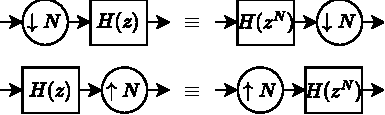
\includegraphics[keepaspectratio, scale=0.9]
            {\currfiledir/figs/Noble_Identity.pdf}
            \caption{Noble Identity}
            \label{figure:Noble_Identity}
        \end{figure}
    \section{導出}
        \begin{proof}
            \quad\par\noindent
            (オーバー・サンプリングの場合)
            \par\noindent
            \cref{figure:Noble_Identity} の下段に着目する。
            システム $\SH$ のインパルス応答を $h:\integers\to\complexNumbers$ とする。
            $\SH$ は因果的なシステムであるとする$\parens{\forall n<0,\;h(n)=0}$。
            z 変換が $\tilde{H}:z\mapsto H(z^N)$ で与えられるシステム $\StH$ のインパルス応答を $\tilde{h}:\integers\to\complexNumbers$ とすると, z 変換の定義から次式が成り立つ。
            \[
                \tilde{h}(n) = \begin{cases}
                    h(n/N) & (N\mid n) \\
                    0 & (N\nmid n)
                \end{cases} \tag{1}
            \]
            図の左側のシステムに於いて,入力を $x:\integers\to\complexNumbers$,$\SH$ の出力を $\xLone:\integers\to\complexNumbers$,最終出力を $\yL:\integers\to\complexNumbers$ とすると次式が成り立つ。
            \begin{align*}
                \xLone(n) &= (h*x)(n) = \sum_{m=0}^\infty h(m)x(n-m) \\
                \yL(n) &= \begin{cases}
                    \xLone(n/N) & (N\mid n) \\
                    0 & (N\nmid n)
                \end{cases} \\
                &= \begin{cases}
                    \sum_{m=0}^\infty h(m)x(n/N-m) & (N\mid n) \\
                    0 & (N\nmid n)
                \end{cases}
            \end{align*}
            図の右側のシステムに於いて,$\uparrow N$ の出力を $\xRone$,最終出力を $\yR$ とすると次式が成り立つ。
            \begin{align*}
                \xRone(n) &= \begin{cases}
                    x(n/N) & (N\mid n) \\
                    0 & (N\nmid n)
                \end{cases} \\
                \yR(n) &= (\tilde{h}*\xRone)(n) = \sum_{m=0}^\infty \tilde{h}(m)\xRone(n-m) \\
                &= \sum_{l=0}^\infty \tilde{h}(lN)\xRone(n-lN) = \sum_{l=0}^\infty h(l)\xRone(n-lN) \\
                &= \begin{cases}
                    \sum_{l=0}^\infty h(l)x(n/N-l) & (N\mid n) \\
                    0 & (N\nmid n)
                \end{cases}
            \end{align*}
            $\yL$ と $\yR$ は一致する。
            \newline
            \quad\par\noindent
            (アンダー・サンプリングの場合)
            \par\noindent
            \cref{figure:Noble_Identity} の上段に着目する。
            断りの無い限り,「(オーバー・サンプリングの場合)」で定義した記号の意味を引き継ぐ。
            図の左側のシステムに於いて,入力を $x:\integers\to\complexNumbers$,$\downarrow N$ の出力を $\xLone:\integers\to\complexNumbers$,最終出力を $\yL:\integers\to\complexNumbers$ とすると次式が成り立つ。
            \begin{align*}
                \xLone(n) &= x(nN) \\
                \yL(n) &= \sum_{m=0}^\infty h(m)\xLone(n-m) = \sum_{m=0}^\infty h(m)x((n-m)N)
            \end{align*}
            図の右側のシステムに於いて,$\StH$ の出力を $\xRone$,最終出力を $\yR$ とすると次式が成り立つ。
            \begin{align*}
                \xRone(n) &= \sum_{m=0}^\infty \tilde{h}(m)x(n-m) = \sum_{l=0}^\infty \tilde{h}(lN)x(n-lN) = \sum_{l=0}^\infty h(l)x(n-lN) \\
                \yR(n) &= \xRone(nN) = \sum_{l=0}^\infty h(l)x((n-l)N)
            \end{align*}
            $\yL$ と $\yR$ は一致する。
        \end{proof}
